\documentclass[12pt,a4paper]{article}
\usepackage[a4paper,top=22mm,bottom=24mm,left=22mm,right=22mm]{geometry}
\usepackage{graphicx,booktabs,longtable,array,float,xcolor,hyperref,caption,enumitem}
\usepackage{xepersian}
\settextfont{Tahoma}
\setlatintextfont{Times New Roman}
\setdigitfont{Tahoma}
\graphicspath{{figures/}}
\hypersetup{colorlinks=true,linkcolor=blue!45!black,urlcolor=blue!55!black}
\captionsetup{font=small,labelfont=bf}
\setlength{\parskip}{0.55em}
\setlength{\parindent}{0pt}
\renewcommand{\arraystretch}{1.25}

\title{\textbf{گزارش تحلیل بازار فیزیکی و حباب گواهی سپرده گندله سنگ‌آهن}}
\author{پروژه پژوهش کالایی گندله}
\date{آخرین به‌روزرسانی: ۲۴ مرداد ۱۴۰۵}

\begin{document}
\maketitle
\thispagestyle{empty}

\begin{center}
\colorbox{blue!6}{\begin{minipage}{0.90\textwidth}
\textbf{پرسش پژوهش:}
گواهی سپرده گندله سنگ‌آهن نسبت به یک معیار قابل‌دفاع از معاملات داخلی گندله
با چه میزان صرف یا تخفیف معامله می‌شود؟

\textbf{محدوده:}
این گزارش صرفاً قیمت گواهی را با معاملات داخلی بازار فیزیکی مقایسه می‌کند.
ارزش‌گذاری مبتنی بر قیمت جهانی، نرخ ارز یا مدل ارزش ذاتی خارجی در دامنه پژوهش نیست.
\end{minipage}}
\end{center}

\newpage
\tableofcontents
\newpage

\section{خلاصه مدیریتی}

داده گواهی سپرده و بازار فیزیکی از منابع رسمی بورس کالای ایران جمع‌آوری و بدون
تغییر در لایه خام نگهداری شده‌اند. برای انتخاب نماینده بازار، حجم همه معاملات
مثبت فیزیکی از شروع معاملات گواهی بررسی شد. گل‌گهر و گهرزمین با سهم ترکیبی
۵۳٫۸۶ درصد انتخاب شدند. چادرملو و سنگان خراسان به دلیل سهم حجمی به‌مراتب کمتر
و سهم ترکیبی ۱۵٫۴۷ درصد از معیار قیمت حذف شدند.

قیمت فیزیکی فقط از معاملات دارای قرارداد نقدی یا نقدی مچینگ، تسویه کاملاً نقدی،
قیمت مثبت و مقدار مثبت ساخته شد. هر روزی که حداقل یکی از دو شرکت منتخب معامله
کرده باشد معتبر است: در روز تک‌شرکتی قیمت همان شرکت و در روز دوشرکتی میانگین
ساده قیمت دو شرکت استفاده می‌شود. مقایسه با گواهی فقط در تاریخ دقیق انجام شده
و هیچ قیمت کهنه، میان‌یابی یا انتقال قیمت روز قبل به کار نرفته است.

نمونه نهایی شامل ۲۲ روز است: ۱۶ روز تک‌شرکتی و ۶ روز دوشرکتی. میانگین حباب
۱۲٫۱۸ درصد منفی و میانه آن ۱۱٫۵۵ درصد منفی است. فقط یک مشاهده مثبت، در
۱۴۰۴/۱۰/۲۱، وجود دارد. نتیجه اصلی این مرحله آن است که گواهی در اغلب نقاط
قابل‌مقایسه با تخفیف نسبت به معیار فیزیکی معامله شده است؛ بااین‌حال غلبه
روزهای تک‌شرکتی، نتیجه‌گیری ساختاری درباره اندازه بلندمدت حباب را محدود می‌کند.

\begin{table}[H]
\centering
\caption{شاخص‌های اصلی مطالعه}
\begin{tabular}{lr}
\toprule
شاخص & مقدار \\
\midrule
ردیف‌های خام بازار فیزیکی & ۳٬۴۶۷ \\
معاملات مثبت بازار فیزیکی & ۱٬۶۰۶ \\
روزهای معامله مثبت گواهی & ۱۸۲ \\
نقاط دقیق حباب & ۲۲ \\
روزهای تک‌شرکتی & ۱۶ \\
روزهای دوشرکتی & ۶ \\
میانگین حباب & ۱۲٫۱۸\%- \\
میانه حباب & ۱۱٫۵۵\%- \\
کمینه حباب & ۲۴٫۹۳\%- \\
بیشینه حباب & ۱۱٫۰۳\%+ \\
\bottomrule
\end{tabular}
\end{table}

\section{منابع داده و معماری}

\subsection{گواهی سپرده}
سری گواهی از API رسمی CDC بورس کالای ایران، بازار ۲۲، دریافت شده است. دو کد
\lr{CD1IOP0001} و \lr{IronOrePlt} یک سری پیوسته را تشکیل می‌دهند. تاریخ شروع
سری ۱۴۰۴/۰۷/۲۸ است و قیمت معیار گواهی \lr{TodaySettlementPrice} است. نسبت
ارزش به حجم صرفاً برای کنترل سازگاری قیمت استفاده می‌شود.

\subsection{بازار فیزیکی}
داده بازار فیزیکی از API رسمی آمار معاملات بورس کالا گردآوری شده و دامنه خام
تمام ردیف‌های نرمال‌شده با نام «گندله سنگ آهن» را حفظ می‌کند. فیلتر تولیدکننده،
نوع قرارداد، شیوه تسویه و معامله مثبت فقط در لایه تحلیل اعمال شده است.

\subsection{اصول نگهداری و بازتولید}
\begin{itemize}[rightmargin=1.5em]
  \item فایل‌های خام و snapshotها immutable هستند و تحلیل آنها را بازنویسی نمی‌کند.
  \item collectorها incremental، idempotent و atomic طراحی شده‌اند.
  \item شکل‌ها با \lr{reports/build\_report\_figures.py} از CSVهای خام ساخته می‌شوند.
  \item notebook اصلی \lr{notebooks/01\_physical\_analysis.ipynb} است.
\end{itemize}

\section{انتخاب تولیدکنندگان}

برای جلوگیری از انتخاب یک معیار کم‌نماینده، سهم تولیدکنندگان در \textbf{همه
معاملات مثبت فیزیکی} از شروع گواهی محاسبه شد؛ غربالگری به نوع قرارداد یا
شیوه تسویه محدود نیست. حجم کل بازار در این بازه ۱۰٬۷۵۱٬۰۰۰ تن است.

\begin{table}[H]
\centering
\caption{نمایندگی حجمی تولیدکنندگان مورد بررسی}
\begin{tabular}{lrr}
\toprule
تولیدکننده & حجم (تن) & سهم از کل بازار \\
\midrule
گل‌گهر & ۳٬۳۰۶٬۰۰۰ & ۳۰٫۷۵\% \\
گهرزمین & ۲٬۴۸۴٬۰۰۰ & ۲۳٫۱۰\% \\
چادرملو & ۱٬۰۵۵٬۰۰۰ & ۹٫۸۱\% \\
سنگان خراسان & ۶۰۸٬۰۰۰ & ۵٫۶۶\% \\
\midrule
گل‌گهر و گهرزمین & ۵٬۷۹۰٬۰۰۰ & ۵۳٫۸۶\% \\
چادرملو و سنگان & ۱٬۶۶۳٬۰۰۰ & ۱۵٫۴۷\% \\
\bottomrule
\end{tabular}
\end{table}

\begin{figure}[H]
\centering
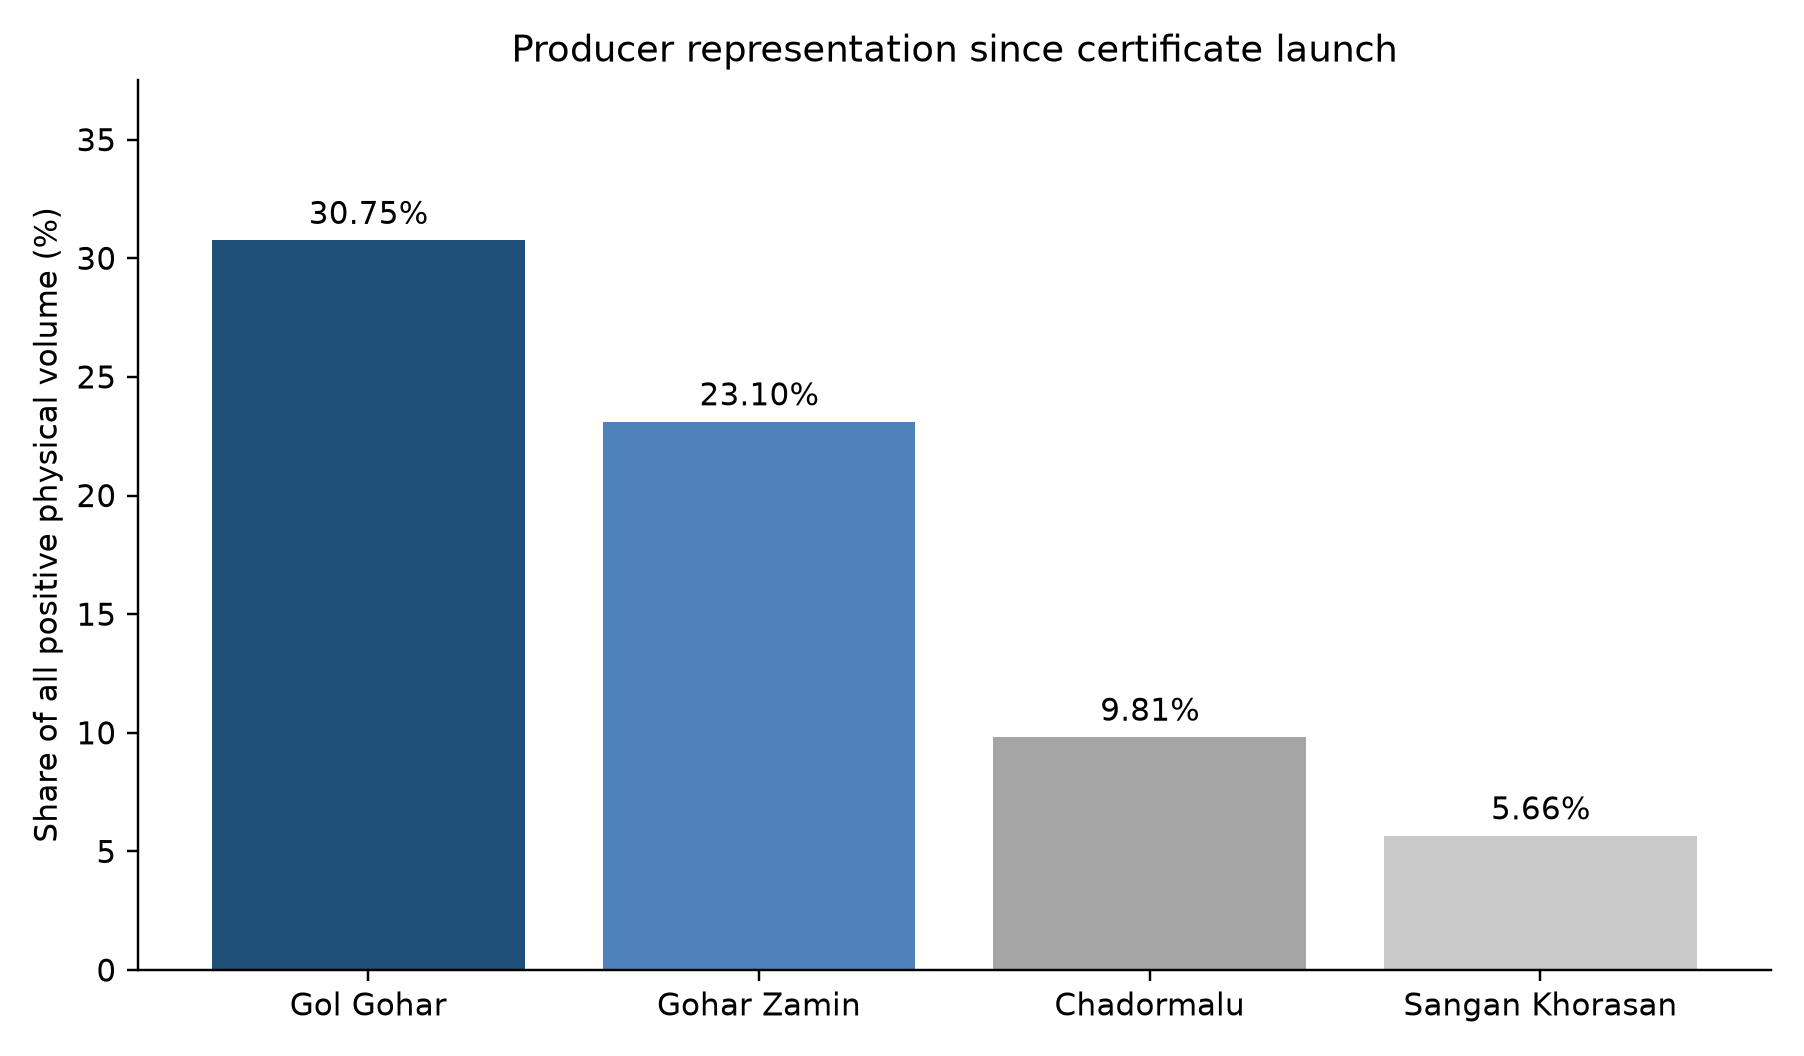
\includegraphics[width=0.86\textwidth]{producer_market_share.png}
\caption{سهم حجمی چهار تولیدکننده از همه معاملات مثبت بازار پس از شروع گواهی}
\end{figure}

گل‌گهر و گهرزمین به دلیل سهم ترکیبی ۵۳٫۸۶ درصد و نزدیکی بیشتر رفتار قیمتی
انتخاب شدند. چادرملو و سنگان حذف تحلیلی شدند، زیرا بازار غالب در اختیار آنها
نیست و هر یک سهمی بسیار کمتر از دو رهبر بازار دارند. داده آنها از raw حذف نشده
و برای audit محفوظ است.

\section{تعریف نهایی قیمت فیزیکی}

یک ردیف فقط زمانی وارد محاسبه قیمت می‌شود که نوع قرارداد «نقدی» یا «نقدی
(مچینگ)»، شیوه تسویه دقیقاً «نقدی»، قیمت و مقدار مثبت، و نماد متعلق به یکی از
دو شرکت منتخب باشد.

اگر یک شرکت در یک روز چند ردیف واجد شرایط داشته باشد:
\[
P_{i,t}=\frac{\sum_j P_{i,t,j}Q_{i,t,j}}{\sum_j Q_{i,t,j}}
\]

معیار فیزیکی روزانه از اجتماع روزهای معامله دو شرکت ساخته می‌شود:
\[
P^{physical}_t =
\begin{cases}
P_{GOLG,t} & \text{فقط گل‌گهر موجود باشد}\\
P_{GHZ,t} & \text{فقط گهرزمین موجود باشد}\\
\dfrac{P_{GOLG,t}+P_{GHZ,t}}{2} & \text{هر دو موجود باشند}
\end{cases}
\]

در روز دوشرکتی میانگین ساده انتخاب شده است. روز بدون معامله هر دو شرکت فاقد
benchmark است.

\begin{figure}[H]
\centering
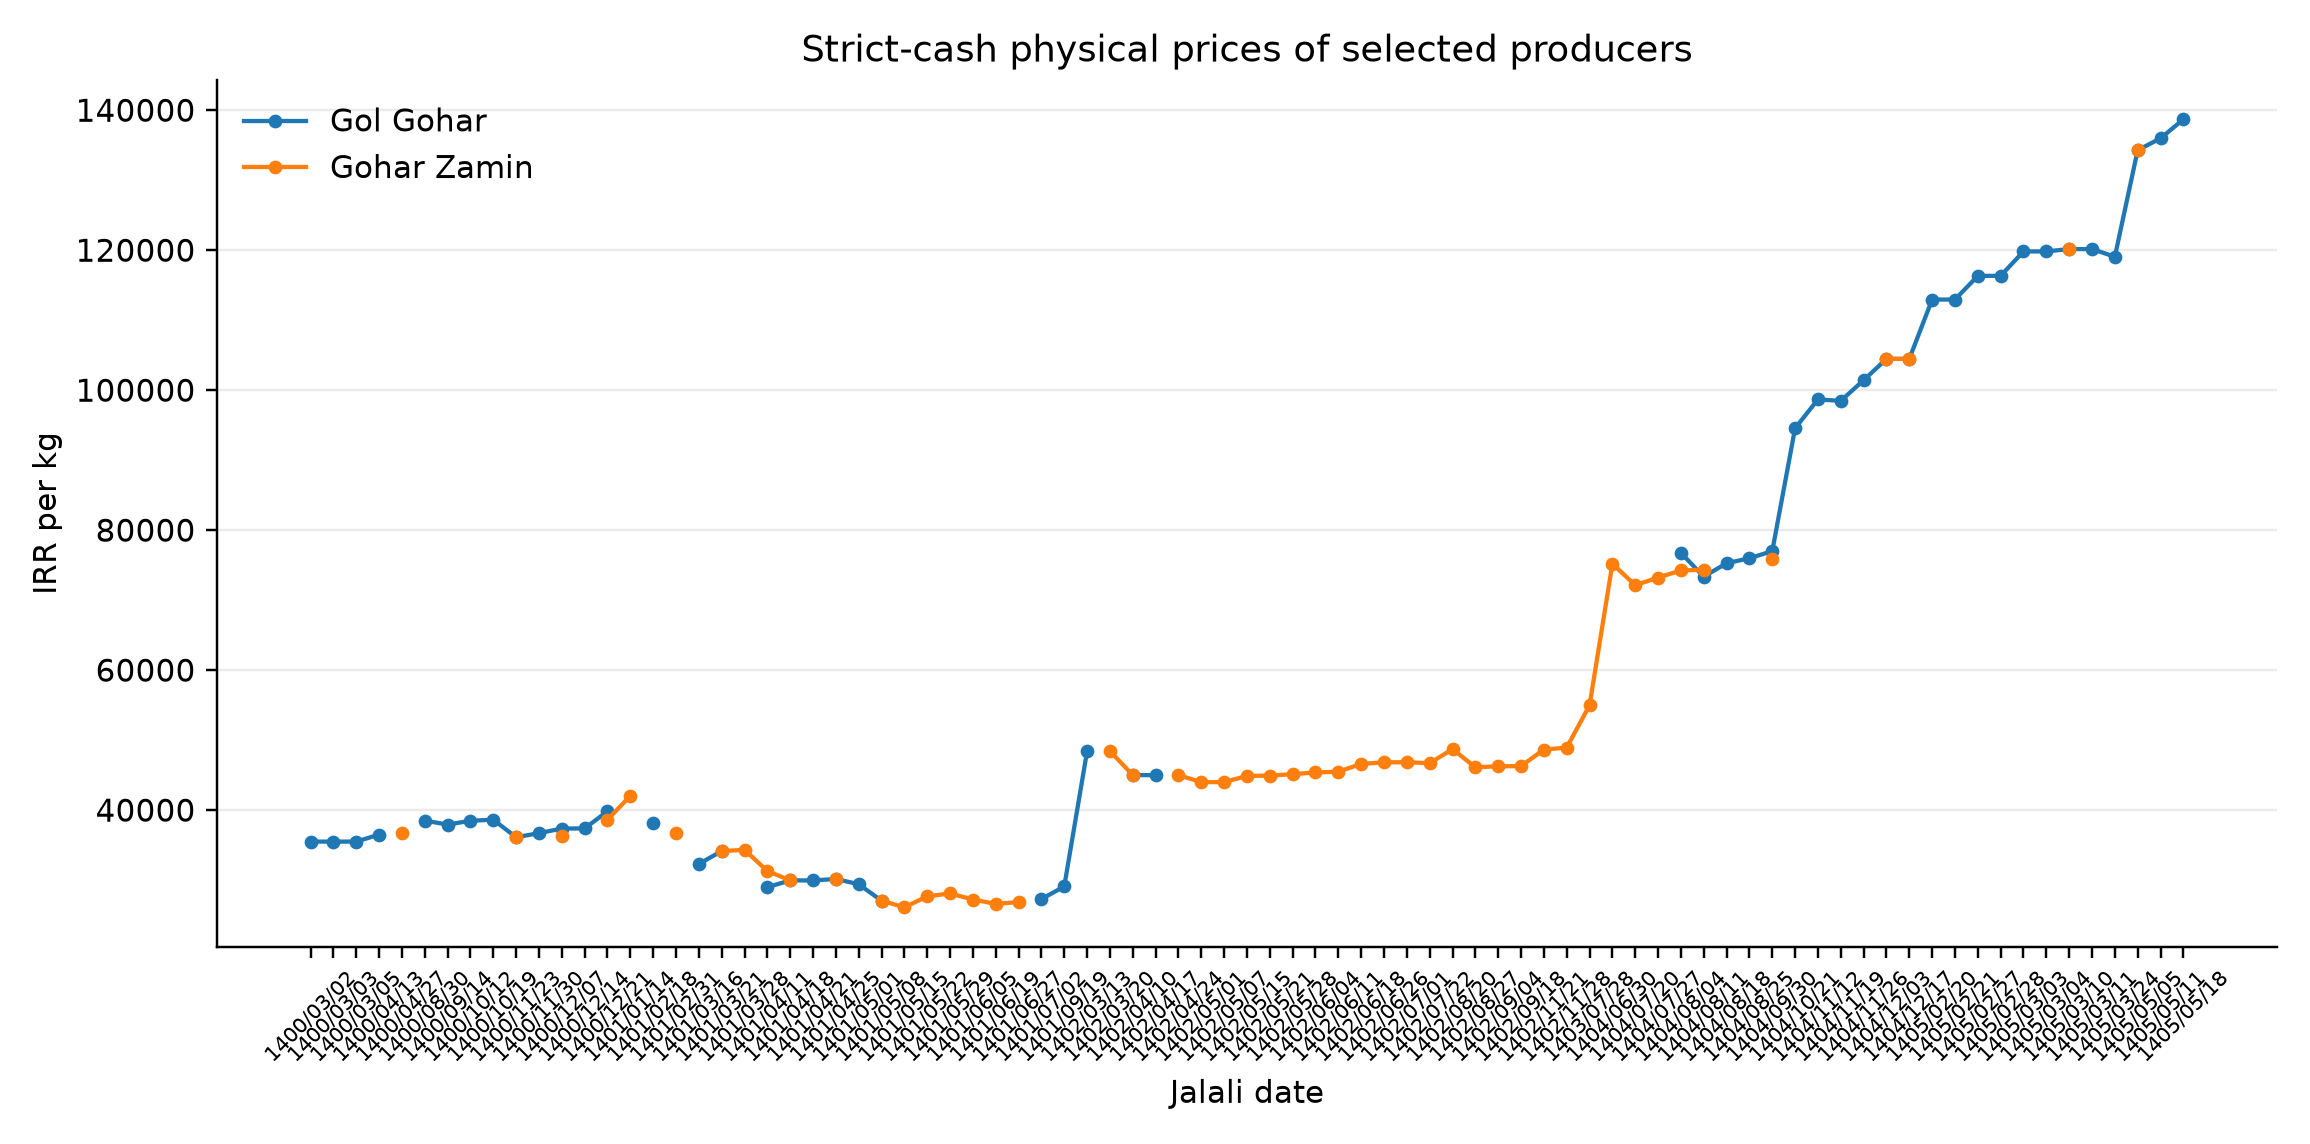
\includegraphics[width=0.94\textwidth]{selected_physical_prices.png}
\caption{مسیر قیمت نقدی واقعی گل‌گهر و گهرزمین در دامنه کامل داده}
\end{figure}

\section{بررسی همگنی قیمت دو شرکت}

در کل تاریخ ۱۶ روز معامله نقدی واقعی مشترک وجود دارد: ۹ روز پیش از شروع گواهی
و ۷ روز پس از آن. اختلاف متقارن از رابطه زیر محاسبه شد:
\[
D^{sym}_t =
100\times\frac{|P_{GOLG,t}-P_{GHZ,t}|}{(P_{GOLG,t}+P_{GHZ,t})/2}
\]

\begin{table}[H]
\centering
\caption{خلاصه اختلاف قیمت در روزهای مشترک}
\begin{tabular}{lrr}
\toprule
دوره & تعداد روز & متوسط اختلاف متقارن \\
\midrule
قبل از شروع گواهی & ۹ & ۱٫۵۳\% \\
بعد از شروع گواهی & ۷ & ۰٫۸۸\% \\
\bottomrule
\end{tabular}
\end{table}

میانه اختلاف در هر دو دوره صفر است. پس از شروع گواهی در ۴ روز از ۷ روز مشترک،
قیمت دو شرکت دقیقاً برابر بوده و بیشترین اختلاف متقارن ۳٫۳۲ درصد است. بنابراین
شواهدی مبنی بر افزایش واگرایی قیمت دو شرکت پس از شروع گواهی وجود ندارد.

\section{فرمول و نتایج حباب}

حباب جهت‌دار فقط در روز دارای معامله مثبت گواهی و benchmark همان تاریخ محاسبه می‌شود:
\[
Bubble_t=100\times\left(\frac{P^{certificate}_t}{P^{physical}_t}-1\right)
\]
عدد مثبت premium و عدد منفی discount است. هیچ انتقال قیمت یا میان‌یابی انجام نمی‌شود.

\begin{figure}[H]
\centering
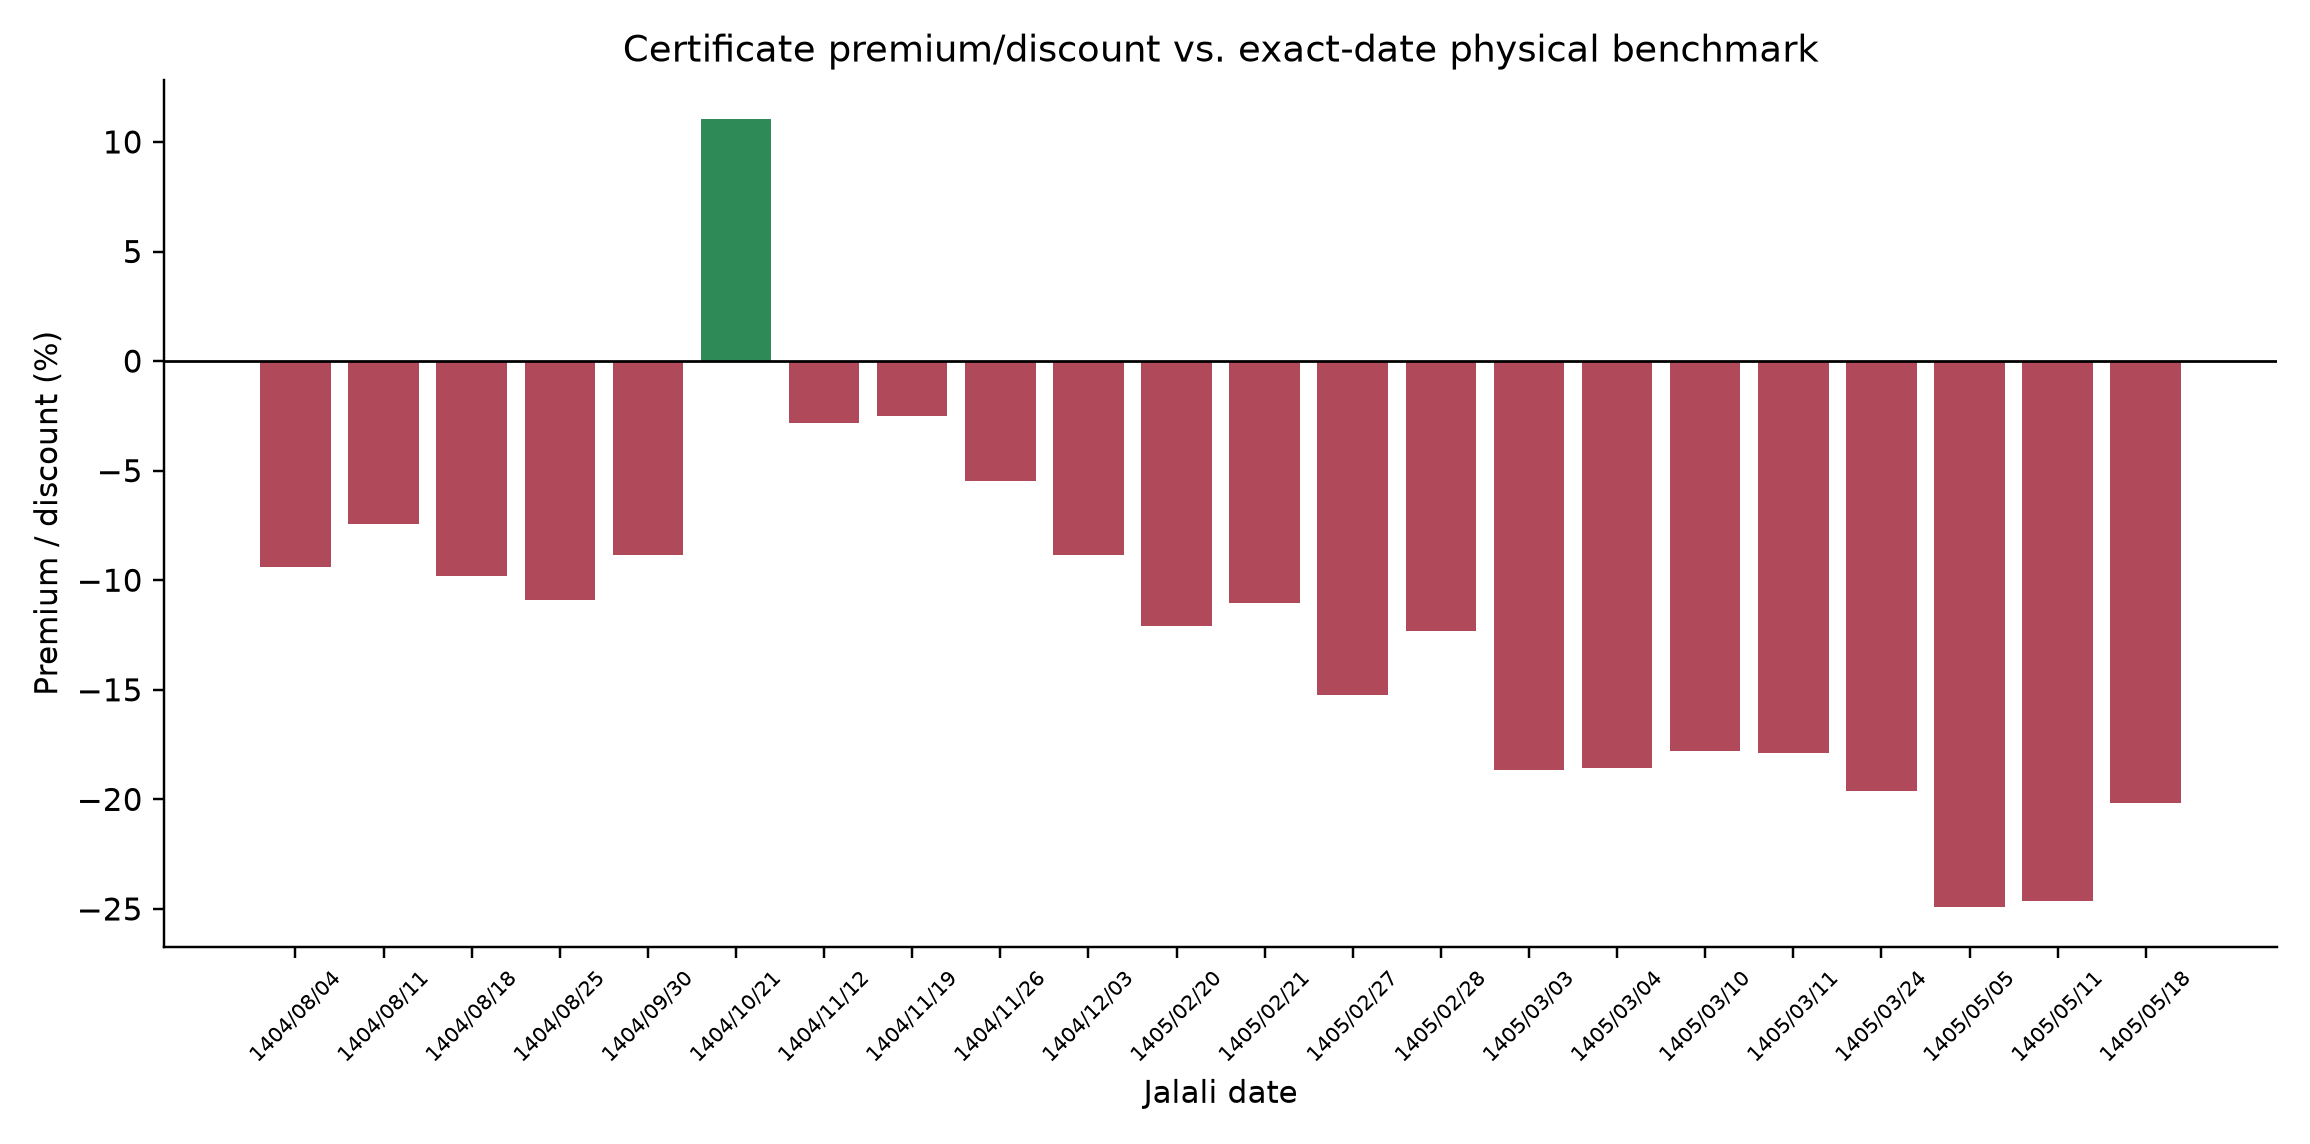
\includegraphics[width=0.96\textwidth]{certificate_bubble.png}
\caption{حباب گواهی نسبت به معیار فیزیکی در ۲۲ تاریخ دقیق مشترک}
\end{figure}

\subsection{جدول کامل مشاهدات}
\begin{longtable}{rrrrr}
\caption{تمام نقاط دقیق تحلیل حباب}\\
\toprule
تاریخ & معیار فیزیکی & تسویه گواهی & حباب & شرکت \\
\midrule
\endfirsthead
\toprule
تاریخ & معیار فیزیکی & تسویه گواهی & حباب & شرکت \\
\midrule
\endhead
۱۴۰۴/۰۸/۰۴ & ۷۵٬۴۹۴٫۵ & ۶۸٬۳۸۸ & ۹٫۴۱\%- & ۲ \\
۱۴۰۴/۰۸/۱۱ & ۷۳٬۸۵۴ & ۶۸٬۳۴۷ & ۷٫۴۶\%- & ۲ \\
۱۴۰۴/۰۸/۱۸ & ۷۵٬۲۷۰ & ۶۷٬۸۸۶ & ۹٫۸۱\%- & ۱ \\
۱۴۰۴/۰۸/۲۵ & ۷۵٬۹۸۵ & ۶۷٬۷۰۸ & ۱۰٫۸۹\%- & ۱ \\
۱۴۰۴/۰۹/۳۰ & ۷۶٬۴۲۷٫۵ & ۶۹٬۶۶۴ & ۸٫۸۵\%- & ۲ \\
۱۴۰۴/۱۰/۲۱ & ۹۴٬۵۶۶ & ۱۰۴٬۹۹۸ & ۱۱٫۰۳\%+ & ۱ \\
۱۴۰۴/۱۱/۱۲ & ۹۸٬۶۷۹ & ۹۵٬۸۸۸ & ۲٫۸۳\%- & ۱ \\
۱۴۰۴/۱۱/۱۹ & ۹۸٬۴۷۴ & ۹۶٬۰۲۸ & ۲٫۴۸\%- & ۱ \\
۱۴۰۴/۱۱/۲۶ & ۱۰۱٬۴۲۸ & ۹۵٬۸۷۱ & ۵٫۴۸\%- & ۱ \\
۱۴۰۴/۱۲/۰۳ & ۱۰۴٬۴۷۱ & ۹۵٬۲۱۸ & ۸٫۸۶\%- & ۲ \\
۱۴۰۵/۰۲/۲۰ & ۱۱۲٬۹۴۸ & ۹۹٬۳۱۸ & ۱۲٫۰۷\%- & ۱ \\
۱۴۰۵/۰۲/۲۱ & ۱۱۲٬۹۴۸ & ۱۰۰٬۴۸۴ & ۱۱٫۰۴\%- & ۱ \\
۱۴۰۵/۰۲/۲۷ & ۱۱۶٬۳۳۶ & ۹۸٬۵۹۸ & ۱۵٫۲۵\%- & ۱ \\
۱۴۰۵/۰۲/۲۸ & ۱۱۶٬۳۳۶ & ۱۰۱٬۹۸۵ & ۱۲٫۳۴\%- & ۱ \\
۱۴۰۵/۰۳/۰۳ & ۱۱۹٬۸۲۶ & ۹۷٬۴۹۰ & ۱۸٫۶۴\%- & ۱ \\
۱۴۰۵/۰۳/۰۴ & ۱۱۹٬۸۲۶ & ۹۷٬۵۸۱ & ۱۸٫۵۶\%- & ۱ \\
۱۴۰۵/۰۳/۱۰ & ۱۲۰٬۱۵۹ & ۹۸٬۷۹۰ & ۱۷٫۷۸\%- & ۲ \\
۱۴۰۵/۰۳/۱۱ & ۱۲۰٬۱۵۹ & ۹۸٬۶۷۳ & ۱۷٫۸۸\%- & ۱ \\
۱۴۰۵/۰۳/۲۴ & ۱۱۹٬۰۶۹ & ۹۵٬۷۲۱ & ۱۹٫۶۱\%- & ۱ \\
۱۴۰۵/۰۵/۰۵ & ۱۳۴٬۲۹۶ & ۱۰۰٬۸۲۱ & ۲۴٫۹۳\%- & ۲ \\
۱۴۰۵/۰۵/۱۱ & ۱۳۵٬۹۷۹ & ۱۰۲٬۴۷۰ & ۲۴٫۶۴\%- & ۱ \\
۱۴۰۵/۰۵/۱۸ & ۱۳۸٬۶۹۹ & ۱۱۰٬۷۱۳ & ۲۰٫۱۸\%- & ۱ \\
\bottomrule
\end{longtable}

\section{مطالعه موردی تنها حباب مثبت: ۱۴۰۴/۱۰/۲۱}

\begin{table}[H]
\centering
\caption{مقطع قیمت بازار در ۱۴۰۴/۱۰/۲۱}
\begin{tabular}{lrl}
\toprule
بخش بازار & قیمت (ریال/کیلوگرم) & وضعیت \\
\midrule
گل‌گهر، نقدی واقعی & ۹۴٬۵۶۶ & benchmark رسمی \\
گواهی سپرده & ۱۰۴٬۹۹۸ & قیمت مورد مقایسه \\
گل‌گهر، سلف نقدی/اعتباری & ۱۰۷٬۳۳۲ & خارج از دامنه \\
گهرزمین، نقدی/اعتباری & ۱۱۱٬۲۲۹ & خارج از دامنه \\
\bottomrule
\end{tabular}
\end{table}

معیار رسمی آن روز تک‌شرکتی است:
\[
100\times\left(\frac{104{,}998}{94{,}566}-1\right)=11.03\%
\]

این افزایش در خود ۲۱ دی آغاز نشد. قیمت تسویه گواهی از ۸۱٬۸۴۴ ریال در ۱۰ دی
به ۱۰۳٬۴۸۳ ریال در ۱۷ دی رسیده بود؛ یعنی حدود ۲۶٫۴ درصد رشد. در ۲۱ دی نیز
۲۰۸٬۷۲۶ واحد گواهی در دامنه ۱۰۳٬۵۰۰ تا ۱۰۵٬۵۶۰ ریال معامله شد و تسویه نسبت
به روز معاملاتی قبل ۶٫۹۹ درصد افزایش یافت. بنابراین مشاهده مثبت ناشی از یک
معامله منفرد کم‌حجم نیست.

\begin{figure}[H]
\centering
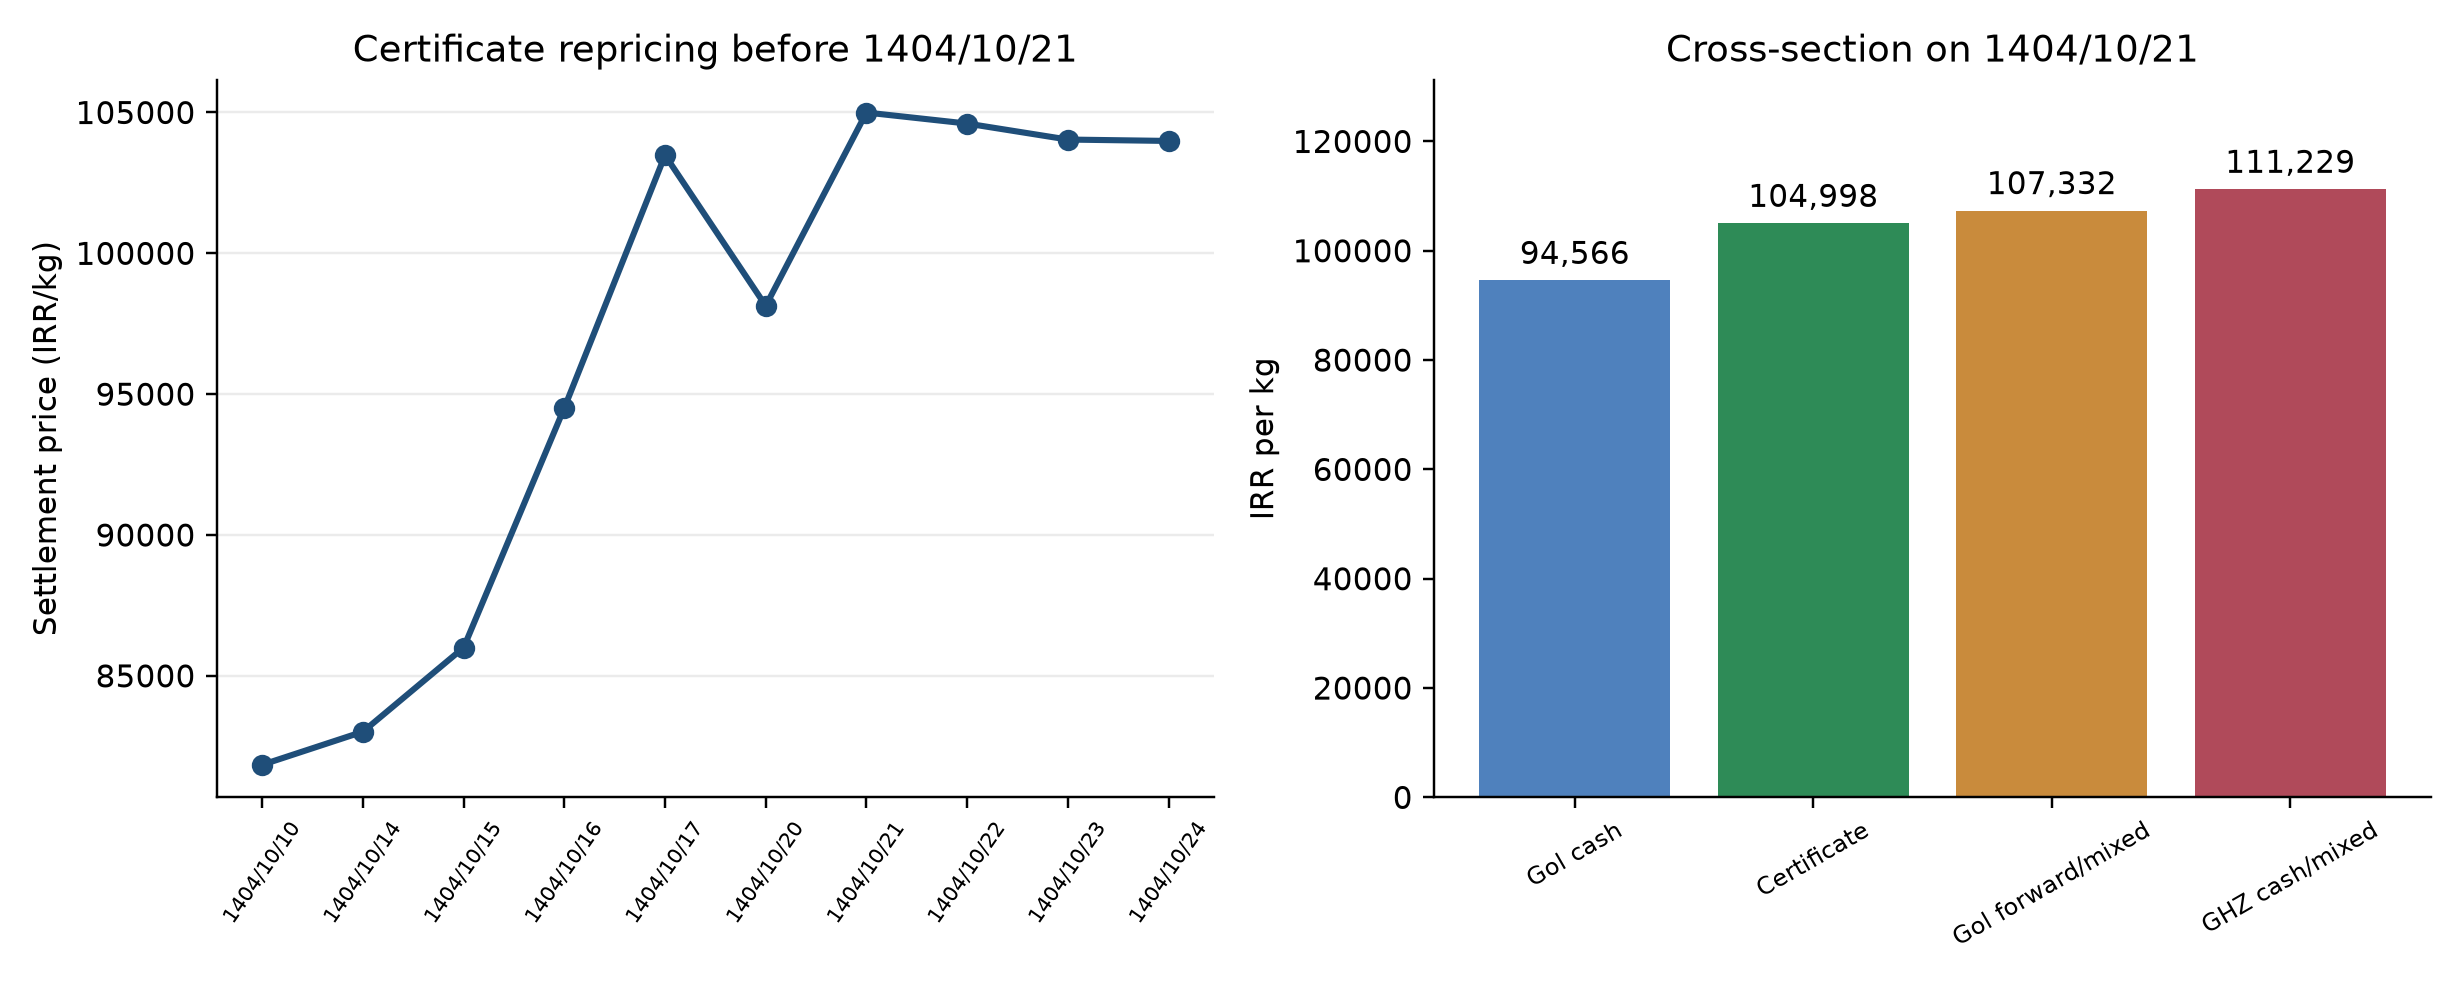
\includegraphics[width=0.98\textwidth]{positive_bubble_case.png}
\caption{مقطع قیمت ۲۱ دی و بازقیمت‌گذاری گواهی پیش از آن تاریخ}
\end{figure}

\subsection{آزمون حساسیت}
قیمت گهرزمین به دلیل تسویه نقدی/اعتباری وارد معیار رسمی نمی‌شود. اگر فقط برای
شناخت حساسیت وارد میانگین شود:
\[
\bar P^{test}=\frac{94{,}566+111{,}229}{2}=102{,}897.5
\]
\[
Bubble^{test}=100\times\left(\frac{104{,}998}{102{,}897.5}-1\right)=2.04\%
\]
حدود ۹ واحد درصد از حباب رسمی به تک‌شرکتی بودن معیار حساس است، ولی علامت مثبت
کاملاً حذف نمی‌شود.

\subsection{تفسیر}
قیمت گواهی میان قیمت نقدی گل‌گهر و قیمت‌های سلف/اعتباری همان روز قرار دارد.
تفسیر محتمل، \textbf{شکاف زمانی کشف قیمت} است: بازار پیوسته گواهی چند روز
زودتر به سطح جدید واکنش نشان داده، درحالی‌که بازار فیزیکی عرضه مقطعی دارد.
بررسی اخبار عمومی، رویداد اختصاصی و هم‌زمانی پیدا نکرد که رابطه علّی مشخصی با
گواهی گندله را اثبات کند. بنابراین این توضیح یک استنباط داده‌محور است، نه علت
بنیادی قطعی. مشاهده حذف نمی‌شود و با برچسب «تک‌شرکتی / حساس به ترکیب» باقی می‌ماند.

\section{محدودیت‌ها}
\begin{enumerate}[rightmargin=1.8em]
  \item تعداد نقاط دقیق فقط ۲۲ روز است.
  \item ۱۶ مشاهده تک‌شرکتی‌اند؛ ترکیب benchmark اهمیت دارد.
  \item کیفیت، محل تحویل، حمل و مزیت نقدشوندگی گواهی در مدل تعدیل نشده‌اند.
  \item نبود خبر اختصاصی به معنی نبود رویداد نیست؛ فقط مانع ادعای علت قطعی است.
  \item این مقایسه بازار داخلی است و نباید ارزش ذاتی تعبیر شود.
\end{enumerate}

\section{نتیجه‌گیری نهایی}
در نمونه موجود، گواهی عمدتاً با discount معامله شده است: میانگین ۱۲٫۱۸ درصد
منفی و میانه ۱۱٫۵۵ درصد منفی. تنها premium مثبت در ۲۱ دی ۱۴۰۴ مشاهده می‌شود.
بخش بزرگ این premium به تک‌شرکتی بودن benchmark حساس است و آزمون حساسیت آن را
از ۱۱٫۰۳ به ۲٫۰۴ درصد کاهش می‌دهد. مسیر زمانی نشان می‌دهد گواهی پیش از آن تاریخ
بازقیمت‌گذاری شده بود؛ بنابراین تفسیر قابل‌دفاع، شکاف زمانی کشف قیمت است.

در گزارش‌های بعدی نتایج باید به تفکیک روزهای تک‌شرکتی و دوشرکتی ارائه شوند.
با افزایش داده، پایداری discount، هزینه حمل و انبار، و تفاوت کیفیت و محل تحویل
باید جداگانه آزمون شود.

\section*{منابع و مسیرهای بازتولید}
\begin{itemize}[rightmargin=1.5em]
  \item \lr{data/raw/certificate/pellet\_certificate\_raw.csv}
  \item \lr{data/raw/physical/pellet\_physical\_raw.csv}
  \item \lr{notebooks/01\_physical\_analysis.ipynb}
  \item \lr{reports/build\_report\_figures.py}
  \item \lr{docs/WORKFLOW.md}
  \item \url{https://sarmayevabourse.ir/20421/}
  \item \url{https://www.sarpoosh.com/economy/stock-market/stock-market1404101408.html}
\end{itemize}

\end{document}
